% Created 2021-02-18 Thu 22:17
% Intended LaTeX compiler: pdflatex
\documentclass[11pt]{article}
\usepackage[utf8]{inputenc}
\usepackage[T1]{fontenc}
\usepackage{graphicx}
\usepackage{grffile}
\usepackage{longtable}
\usepackage{wrapfig}
\usepackage{rotating}
\usepackage[normalem]{ulem}
\usepackage{amsmath}
\usepackage{textcomp}
\usepackage{amssymb}
\usepackage{capt-of}
\usepackage{hyperref}
\date{\today}
\title{}
\hypersetup{
 pdfauthor={},
 pdftitle={},
 pdfkeywords={},
 pdfsubject={},
 pdfcreator={Emacs 28.0.50 (Org mode 9.4.4)}, 
 pdflang={English}}
\begin{document}

\tableofcontents

\section{URL Shortener Design Document}
\label{sec:org6f8958a}

\subsection{Context and scope}
\label{sec:org80bc7fb}
Team:    Alexander, Yaroslav.
Scope:   University assignment.
Project: URL shortener service

The service will allow users to create shorter links and use them instead
of original ones. After link was created, anyone can use it through
this service.
Because this is a university assignment, service will not exhibit any
complex behaviour and instead will do the bare minimum, namely:
\begin{itemize}
\item registration
\item \{un\}authentication
\item creation of short links
\item deletion of short links
\item redirection to the original links
\item own KV(?)-storage
\end{itemize}

\subsubsection{Optimisations and restrictions}
\label{sec:org2c3bb16}
\begin{itemize}
\item Taking into account the absence of e-mail verification, it was decided
to simplify it a bit and allow to use any valid [a-Z0-9]+ string as
a username instead of e-mail.

\item Length of username and password is limited to \$MAX\textsubscript{UNAME}
\$MAX\textsubscript{PW} chars. Length of link is limited to \$MAX\textsubscript{LINK}.
\begin{verbatim}
# size in bytes
MAX_UNAME=32
MAX_PW   =32
MAX_LINK =1024
\end{verbatim}

\item Max number of users - 255, sorry not sorry :(
This derives from `UUID` datatype.
\end{itemize}

\subsection{Goals and non-goals}
\label{sec:org5c0ef54}
The following goals (in somewhat of modified state)
derive from \href{https:https://docs.google.com/document/d/1RIQWpiXRuxUmI\_VhMZjo-UgxMxjEIXIpC2tmMY\_ZpuE}{this} specification.
\begin{enumerate}
\item Snapshot
\label{sec:org95cd483}
\href{specification\_foreign\_2021\_02\_18\_21\_40\_37.pdf}{specification.pdf} downloaded at \textit{[2021-02-18 Thu 21:40]}
\end{enumerate}


\subsubsection{Goals}
\label{sec:orgd4bb57f}
\begin{itemize}
\item User registration
\item User authentication
\item Shortened URLs'  storage
\item Registered users storage
\item Creation and deletion of shortened URLs
\item Url validation before
\item Redirection to the original URL using shortened version
\end{itemize}
\subsubsection{Non-goals}
\label{sec:orgf455ab5}
\begin{itemize}
\item E-mail verification / providing valid e-mail
\item Complex user actions (user data management, password changing, etc\ldots{})
\item UI/GUI/TUI/CLI
\item \ldots{}
\end{itemize}

\subsection{Architecture and Design}
\label{sec:org980e9e8}

\subsubsection{Structs}
\label{sec:org801a30a}
\label{sec:structs}

\begin{verbatim}
type UUID = Word8

data User = User
  { id       :: UUID -- ^ unique ID       -- PK
  , username :: Text -- ^ user's username -- Unique
  , hash     :: Text -- ^ password hash
  }

data Url = Url
  { id    :: UUID -- ^ unique ID                -- PK
  , orig  :: Text -- ^ original url
  , short :: Text -- ^ shortened version of url -- Unique
  , user  :: User -- ^ user that created a link -- FK user(id)
  }
\end{verbatim}

\subsubsection{JWT tokens}
\label{sec:org581c543}
\begin{verbatim}
data Token = Token
  { secret   :: Text
  , username :: Text -- ^ user's username
  }
\end{verbatim}

\subsubsection{Dependencies}
\label{sec:org313cd36}
\begin{itemize}
\item \uline{servant} \texttt{web-server}
\item \uline{colog}   \texttt{logger}
\end{itemize}

\subsubsection{System-context-diagram}
\label{sec:org9d24d86}
\begin{center}
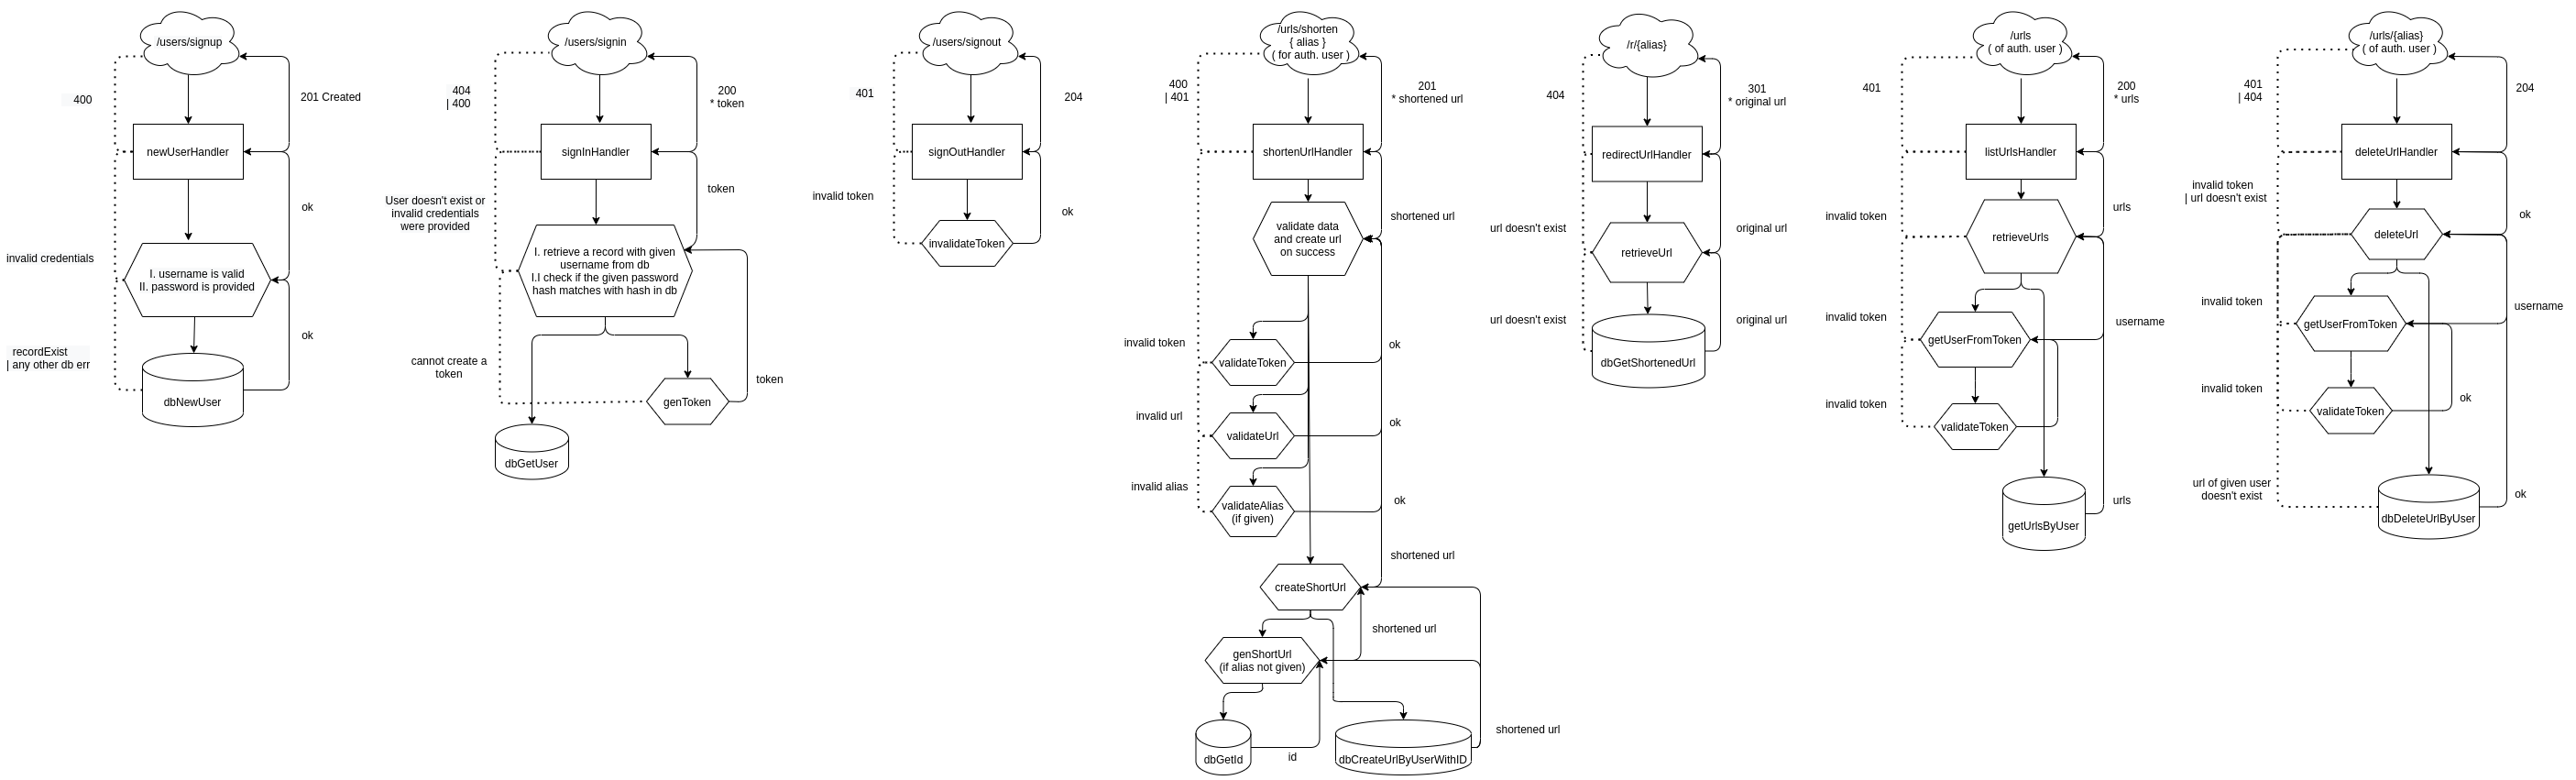
\includegraphics[width=.9\linewidth]{arch.png}
\end{center}

\subsubsection{API}
\label{sec:org776736a}
\url{openapi.yaml}

\begin{itemize}
\item Would be nice to add 409 Conflict (or any other more suitable code)
in /users/signup, when username already exists.
\end{itemize}

\subsubsection{Data Storage}
\label{sec:orgc339f7c}
There are gonna be two tables a.k.a. files:
\begin{itemize}
\item users
\item shortened links
\end{itemize}

Their representation is quiet the same as \hyperref[sec:structs]{datatypes} in haskell.
\begin{enumerate}
\item {\bfseries\sffamily TODO} replace with their \emph{actual} representation.
\label{sec:org3f8c968}

\item {\bfseries\sffamily TODO} describe an algorithm of traversing through the DB
\label{sec:org5c8bad4}
Probably it's gonna be a RB-tree, but need to think about
the implementation part.
\end{enumerate}

\item Common Workflows
\label{sec:org8c2fcc9}
\begin{itemize}
\item insert new user
\item retrieve user credentials
\item generate UUID for new link
\item insert link
\item delete link
\end{itemize}
\end{enumerate}
\end{document}
